
\chapter{Prototype}
\section{Hardware}
\newpage
\section{Software Description}
The software of our \gls{rpi2} consists of two threads and a blocking FileObjectQueue. We get the GPS data from the API and upload it via REST in the Database. 
\subsection{Functions}
First of all a logging property file and a gps property file are loaded. The logging property file contains logging information like the saving location and the maximum number of logging files. The gps property file contains the raspberry id, the server URL and the gps module IP.
\subsection{GPS API}
The API (Gpsd4java) manages the connection with the GPS daemon, which covers receiving data, parsing this information into an useful format and supplying it to the “API Thread”. The GPS data we use consists of the timestamp, coordinateX, coordinateXError, coordinateY, coordinateYError, acceleration, altitude and altitudeError.
\subsection{Tape API}
We implemented this API, because of the problem with saving data into an offline file. This API provides us a FileObjectQueue where we can put and remove our points and this FileObjectQueue is automatically saved in a file. 
\subsection{Save Thread}
The Save thread reads point data from the FileObjectQueue and sends the data to the REST server. When the tracks are written in the database, the Save Thread removes these points from the FileObjectQueue.
\subsection{API Thread}
When the GPS API measures GPS data, the API Thread gets it from the API. The API Thread adds the information about the track and loads it into the FileObjectQueue.
\begin{center}
\includegraphics[width=1\textwidth]{bilder/SoftwareDiagram1}
\end{center} 
\subsection{PHP (REST)}
This part of our software is responsible for the upload into the database. The REST server gets the data formatted as JSON.
\begin{center}
\includegraphics[width=1\textwidth]{bilder/SoftwareDiagram2}
\end{center} 
\section{Code Structure}
\subsection{Classes}
\subsubsection{GPS.java}
\paragraph{Constructor}
In the GPS.java class, the gpsModuleAddress variable is initialized and gets it is value from the GPSConfiguration.java class.
\paragraph{startGpsdClient}
In the startGpsdClient method, the GPS API is initialized and the validate method from the BL.java class is called every time we get data from the GPS API.
\subsubsection{BL.java}
\paragraph{Constructor}
In this class the FileObjectQueue is created and initialized by the save.jPoint file and the GsonConverter.java class. 
Then a new track is created and at last the SaveDataThread object is initialized and started.
\paragraph{Validate}
Checks if the data from the GPS API is a Number if not it will be set to 0 except the latitude and the longitude. If they are NaN it will do nothing. 
Then it adds the data from the GPS API to the FileObjectQueue.
\paragraph{ProcessData}
This method peeks max 50 and min 15 points from the FileObjectQueue and puts them into a JContainer. Then it sends these points to the DataManager.java class to upload them via the uploadContainer method.
\subsubsection{SaveDataThread.java}
This is an intern Class in the BL class which extends Thread.
\paragraph{Run}
This override method calls the ProcessData method and then waits 1 second.
\subsubsection{Data Manager.java}
\paragraph{Constructor}
Gets the server URL and puts it on the urlString variable.
\paragraph{UploadContainer}
Uploads the JContainer it got, to the Server via Rest 
\subsubsection{JContainer.java}
This is a beans class that contains attributes, getter and setter methods for the respective attribute and a toString method of the JContainer.
\subsubsection{JPoint.java}
This is a beans class that contains attributes, getter and setter methods for the respective attribute and a toString method of the JPoint.
\subsubsection{GPSConfiguration.java}
At the beginning this class loads the logging properties.
\paragraph{InitConfiguration}
Reads the properties for the program from a file and sets these values on the specified variables. If a value is not in the file, it sets a default value. And at the end it closes the file.
\subsubsection{GsonConverter.java}
This class is a converter class that has implemented a FileObjectQueue Converter. In the method from, the bytes from the file are converted, so that they can be saved on the FileObjectQueue. In the toStream method, it is the other way round, so the FileObjectQueue is saved on a file.
\subsection{Class Diagram}
\begin{center}
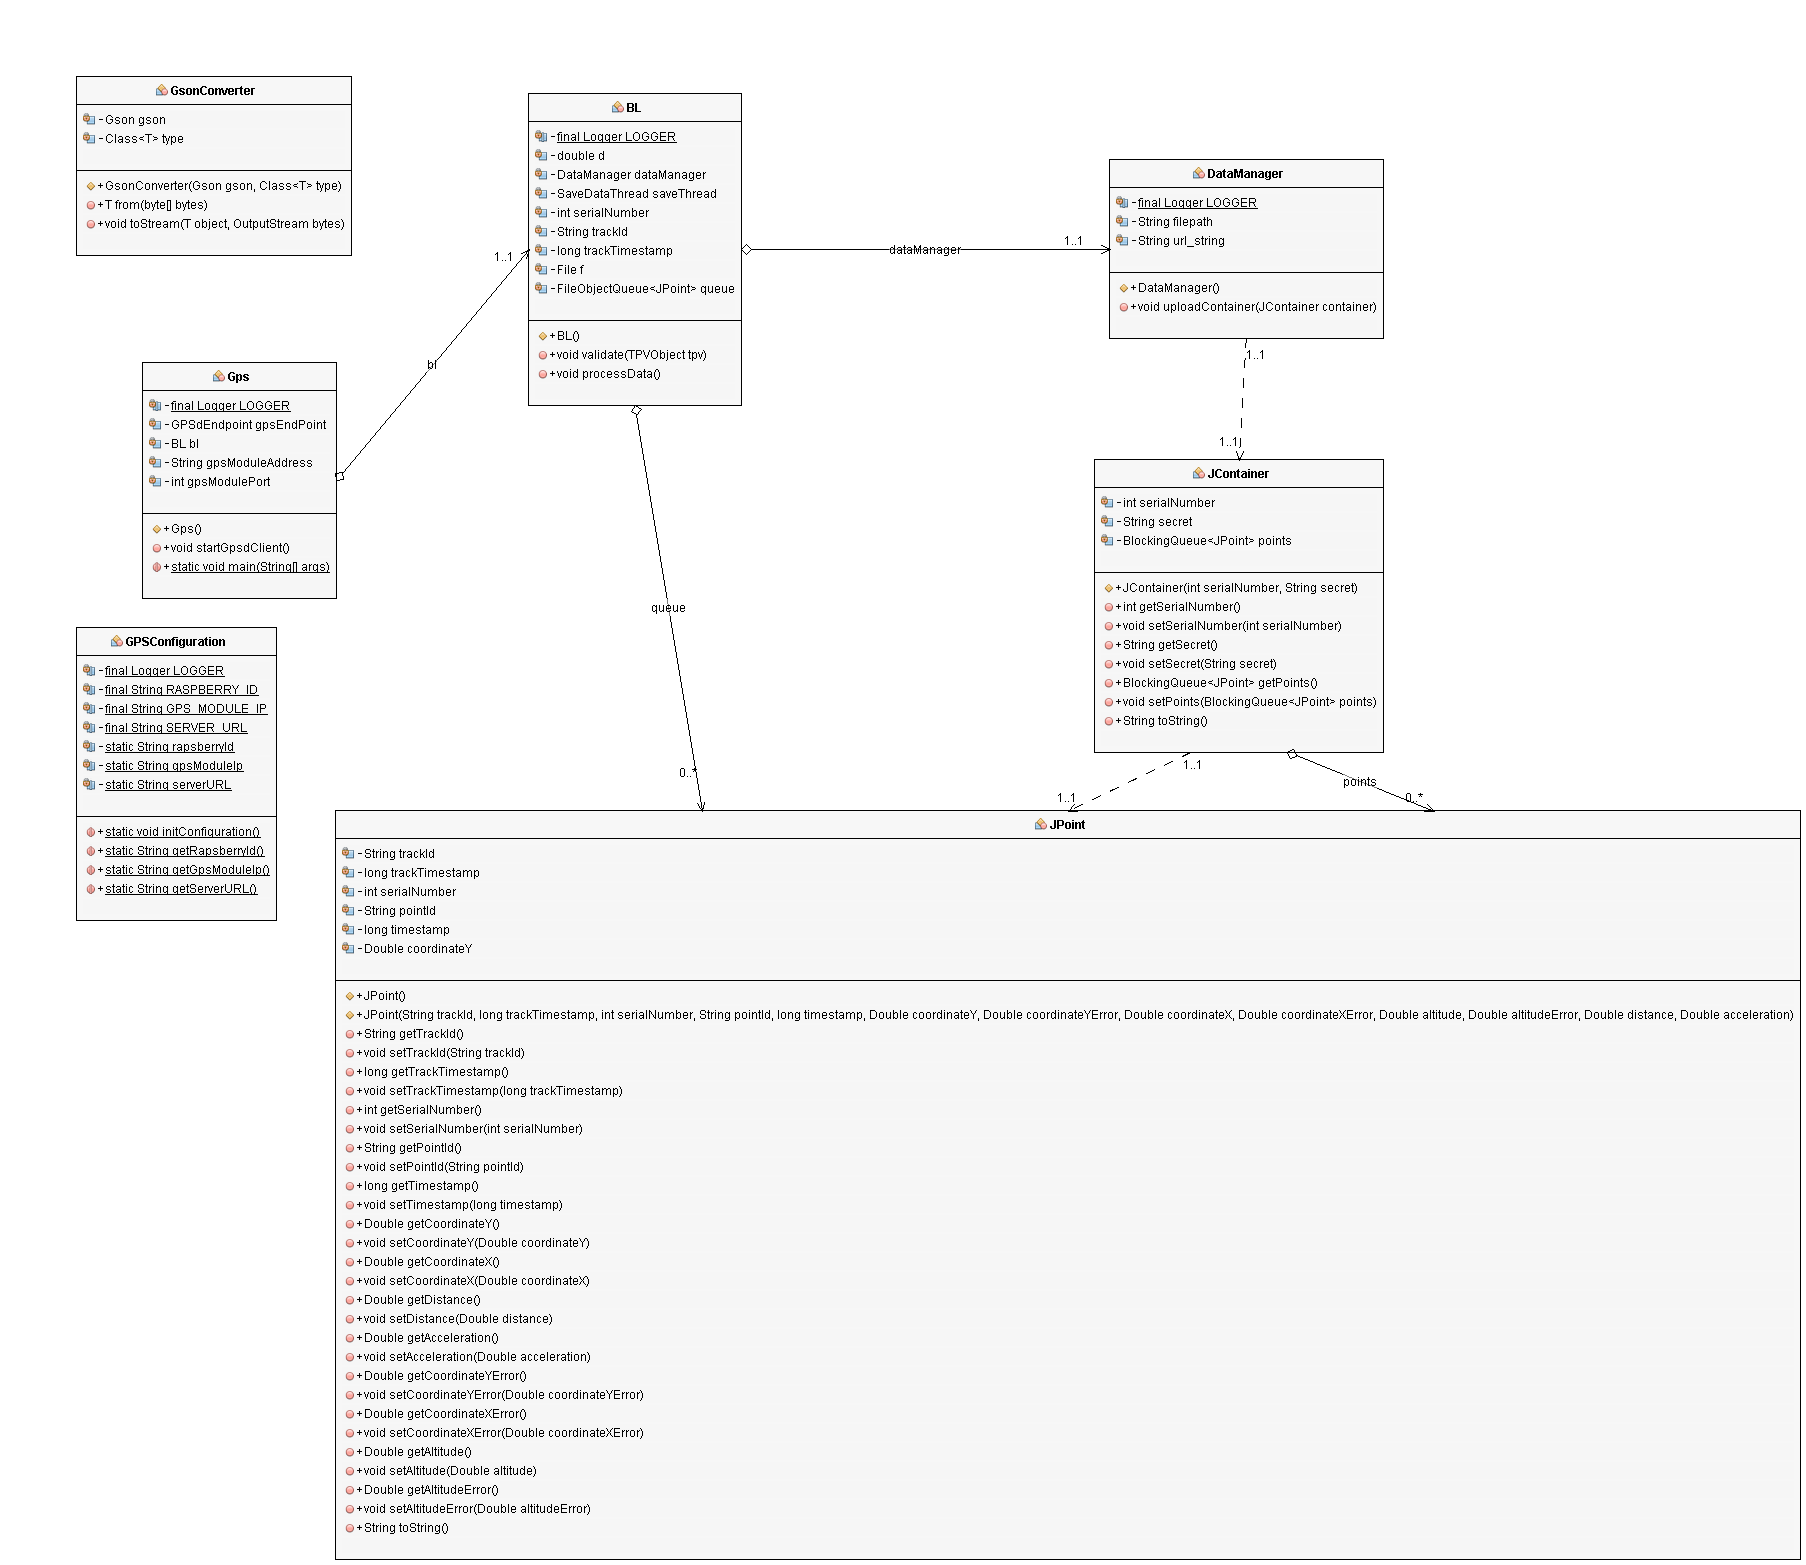
\includegraphics[width=1\textwidth]{bilder/GPS_REST_UML_Diagram}
\end{center}
\section{Problems}
\subsection{Uploading into Database}
When we started with this project, we uploaded tracked data directly into the database over a standard java database connection. During our work on this project, we learned the technology hibernate in school so we reconstructed our program and used hibernate. Later our employer told us, that we should use REST to upload data for a higher security level and fewer connections to the database and therefore less overhead. We wrote the REST php script on our own. 
\subsection{Offline Saving}
When the engine stopped while saving data offline, we had a loss of points, because the whole save file we used was overwritten. So we created a copy of this file, removed the data which was already in the database and deleted the original file. Then we renamed the copy to the original file name. Nevertheless, there was still a problem. On the one hand, it was possible that no data was lost, but on the other hand everything could be lost if the power was cut off between deleting the original file and renaming the copy. This is the reason why we use Tape API now. 
\section{Functional Testing}
To ensure functionality of the hardware prototype and the software, we had to do several tests. They reach from logical problems to practical testing on the road.
\subsection{Database Connection Error}
While developing our software, the error handling when loosing database connection was a very important issue. We had to think about different solutions for different code structure because we changed the database connection type. 
\newline \newline
We decided on the connection type which is called REST. When using the connection which relies on a working connection, there had to be a backup plan if exactly this connection is not working anymore.
\newline \newline
In which cases does an connection error occur:
\begin{itemize}
\item internet not working
\item database not working/running
\end{itemize}

We decided on saving points, which cannot be uploaded, into a JSON (save.jPoint). This solution proved to be the most fitting idea we thought of. It perfectly handled the described problems, reliably managed points and the saving mechanism worked phenomenal.
\newline \newline
The same concept is used when the database is offline or not working properly. 

\subsection{Inaccuracy of the GPS Coordinates}
After the first tests, where we tried to get GPS signal, we noticed the inaccuracy of the signal. This inaccuracy gets influenced by several factors. Therefore we had to find out how precise our GPS coordinates are and how much of an imprecision (part of the GPS data we get from our module) there is. 
\newline \newline
We evaluated driven tracks and measured how much distance there is between the actual location and the GPS coordinates received. This difference was about 5 metres, so no problem at all. 
\newline \newline
Due to the fact that we receive how much of an inaccuracy there is in the GPS data, our partner company can easily extract this information and compensate it in the visualization process. To do that even better, we also saved the deviation and the altitude.

\begin{center}
%grafiken der gefahrenen strecken --> claudio
%\includegraphics[width=1\textwidth]{}
\end{center}

\subsection{No GPS Signal}
When handling the GPS inaccuracy, we had to take into account that there could be no signal at all. Therefore we had to decide on a solution when receiving this data and how to handle and save it.
\newline \newline
We tried different solutions, but finally decided on not saving them. It is the most efficient way concerning storage, both offline and online.
\newline \newline
What does not saving data when having no signal mean for us:
\begin{itemize}
\item when there is no GPS signal, there is often also no internet connection
\item which leads to offline stored “null” points
	\begin{itemize}
	\item not saving these null points is the best solution
	\end{itemize}		
\item data extraction for our partner company when displaying the data on maps will be easier
\end{itemize}